\subsection{Ballmaschine}
\begin{tabular}{p{3.6cm}p{\textwidth-3.6cm-0.7cm}}
\rule{0pt}{11pt}\textit{Typ}              & Ballmaschine \\ 
\rule{0pt}{11pt}\textit{Datum}:           & 18.10.2014   \\
\rule{0pt}{11pt}\textit{Ort}:             & Labor HSLU \\
\rule{0pt}{11pt}\textit{Tester}:          & Gruppe 32 \\
\rule{0pt}{11pt}\textit{Ziel des Testes}: & Das Ziel dieses Testes 
bestand darin, den gebauten Prototyp (Ballmaschine) auf die Genauigkeit 
und Wurfweite zu testen, weitere Erkenntnisse über die Drehzahl der Räder 
zu eruieren. \\
\rule{0pt}{11pt}\textit{Aufbau / Ablauf}: & 
Der Prototyp der Ballmaschine besteht aus zwei Kunststoffrädern mit einer weichen 
Pneubeschichtung. Die Räder sind an einer Metallplatte, direkt auf der 
Welle der Motoren angebracht. Die Motoren sind zwei Gleichstrommotoren, 
welche direkt an ein Netzteil angeschlossen sind. Der Abwurfwinkel ist durch die Stellung 
der Metallplatte gegeben, welche in einem beweglichen Schraubstock 
eingespannt ist. Dadurch können diverse Winkel eingestellt werden. 
Die Zuführung der Bälle erfolgt manuell über eine Schiene. Der Aufbau des Wurfmechanismus ist
in den Abbildungen~\ref{figSub:a} bis~\ref{figSub:c} ersichtlich.\\
\rule{0pt}{11pt}\textit{Fazit / Verbesserungs-\newline vorschlag}: & 
Mit diesem Prototyp konnte gezeigt werden, dass die Flugbahn bei gleichmässiger 
Zuführung sehr konstant ist. Weiter wurde bei einem Abschusswinkel von 45$^\circ$ 
die meisten Treffer erzielt. Ist der Winkel zu klein, so besteht die Gefahr, 
dass die Bälle am Rand des Kübels abprallen. Die Zuführung der Bälle erfolgte 
manuell, welches bei zeitlich ungleicher Berührung der Schwungräder zu grosser 
Wurfdistanzabweichung führte. Dieses kann mit einer automatischen Zuführung behoben 
werden. Beim Abschuss der Bälle werden die Schwungräder immer stark abgebremst. 
Dadurch gibt es bei zu hoher Schussfrequenz eine Abweichung der Wurfweite. Dadurch 
müssen die Bälle gestaffelt abgeschossen werden. Die Abbremsung ist auch von der 
\enquote{Quetschung} der Bälle zwischen den Schwungrädern abhängig. Ist diese sehr 
gross, müssen die Motoren ein viel grösseres Drehmoment aufwenden und brauchen 
dadurch länger um wieder auf die gewünschte Drehzahl zu gelangen. Dies kann über 
den Achsenabstand der Schwungräder eingestellt werden.\newline
%
Die Wurfmaschine kann mit einigen Verbesserungen sehr gute und genaue 
\enquote{Schüsse} erzielen. Zu verbessern sind:
\begin{itemize}
    \item Stabilere Achsen
    \item genauere und gleichmässige Zuführung der Bälle.
    \item einstellbares Grundgerüst
\end{itemize}
\end{tabular}
\begin{figure}[h!]
    \subfigure[Gesamtaufbau\label{figSub:a}]
    {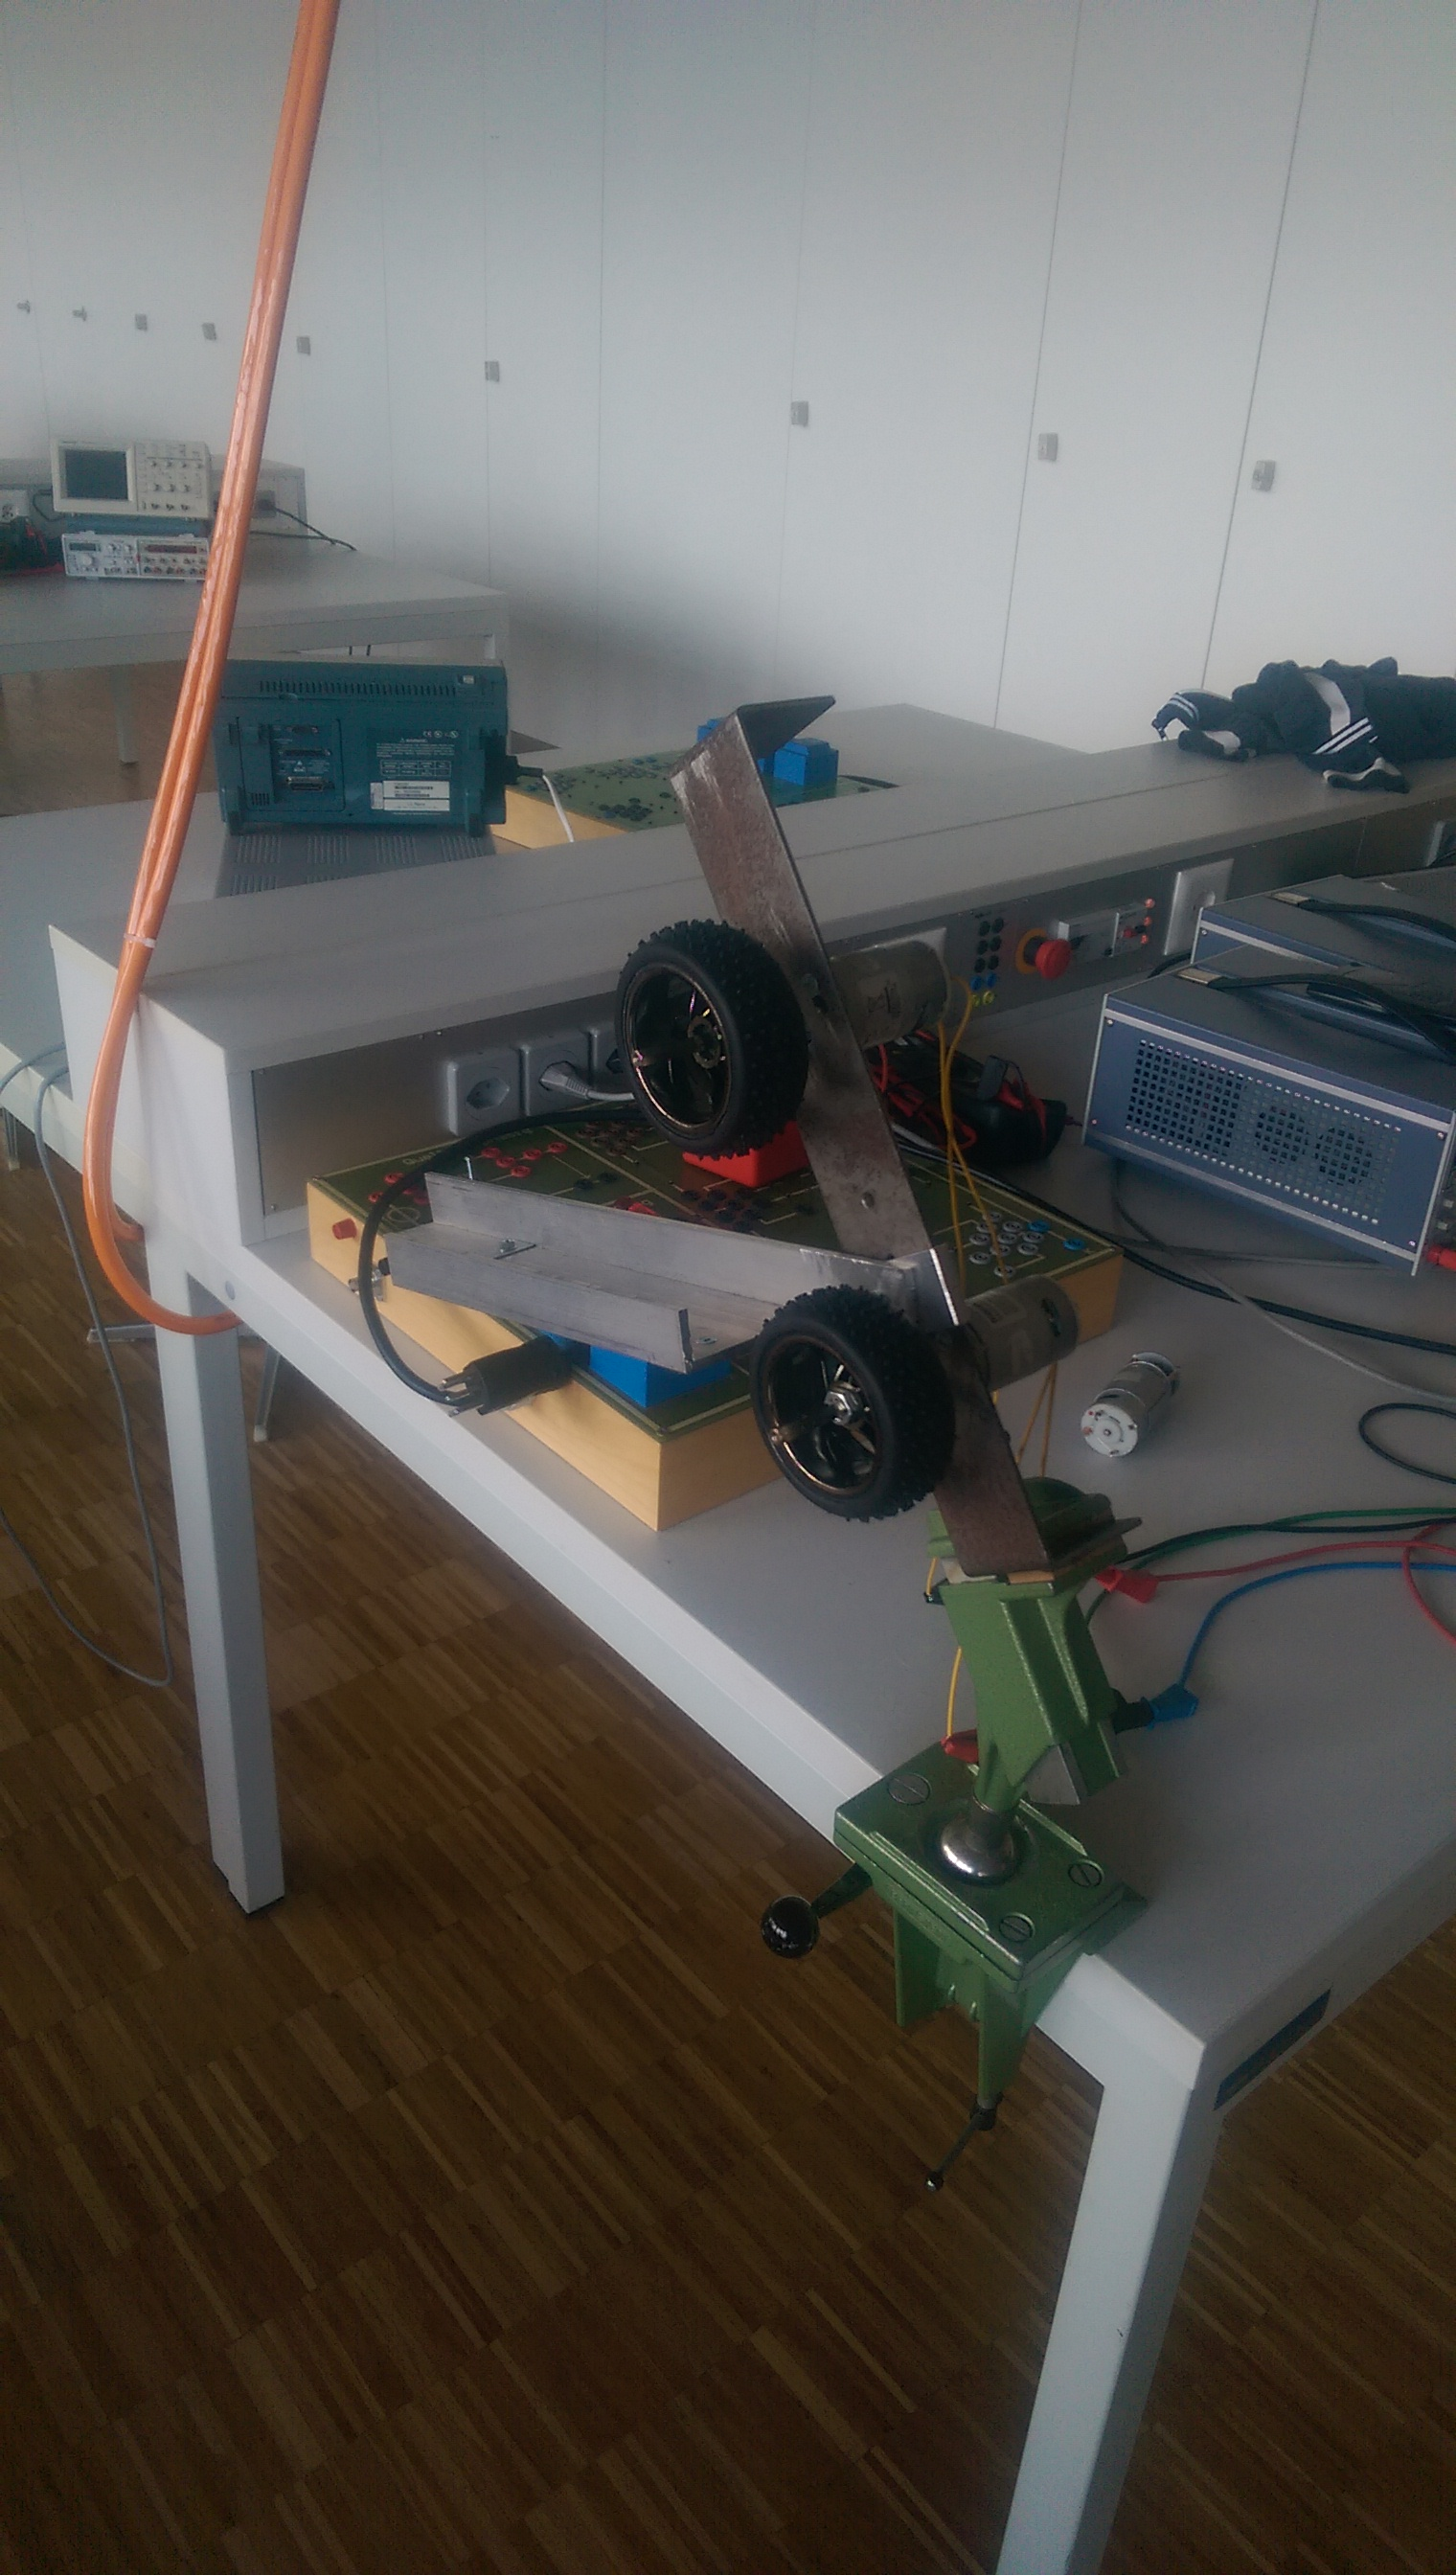
\includegraphics[width=0.6\textwidth,clip,trim=0mm 14cm 0mm 12cm] 
    {Funktionstests/Bilder/Ballmaschine_Drehzahl1.jpg}}
    \hfill
    \subfigure[Funktionsmuster Front Ansicht\label{figSub:b}]
    {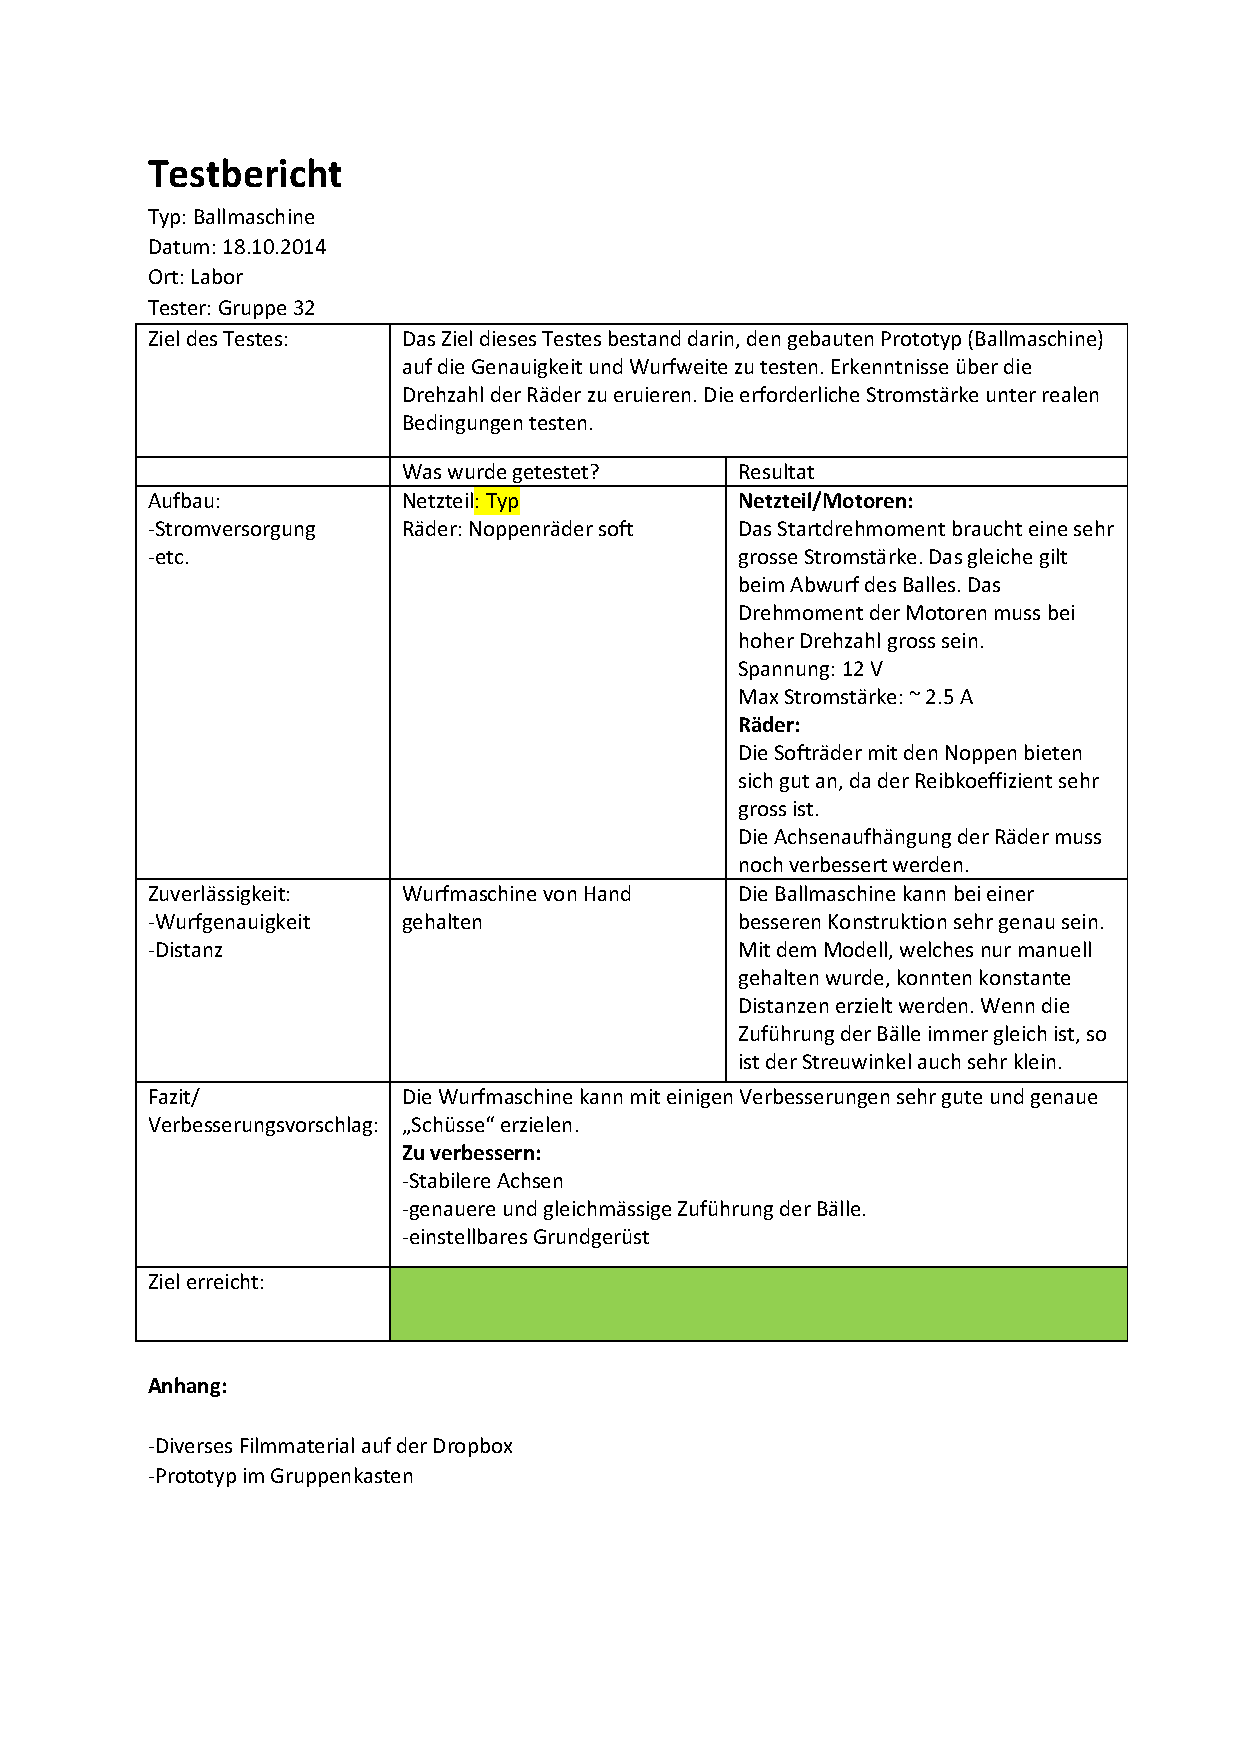
\includegraphics[width=0.35\textwidth,clip,trim=27cm 3cm 0mm 2cm]
    {Funktionstests/Bilder/Ballmaschine.jpg}}
    \vfill
    \subfigure[Funktionsmuster Ballmaschine\label{figSub:c}]
    {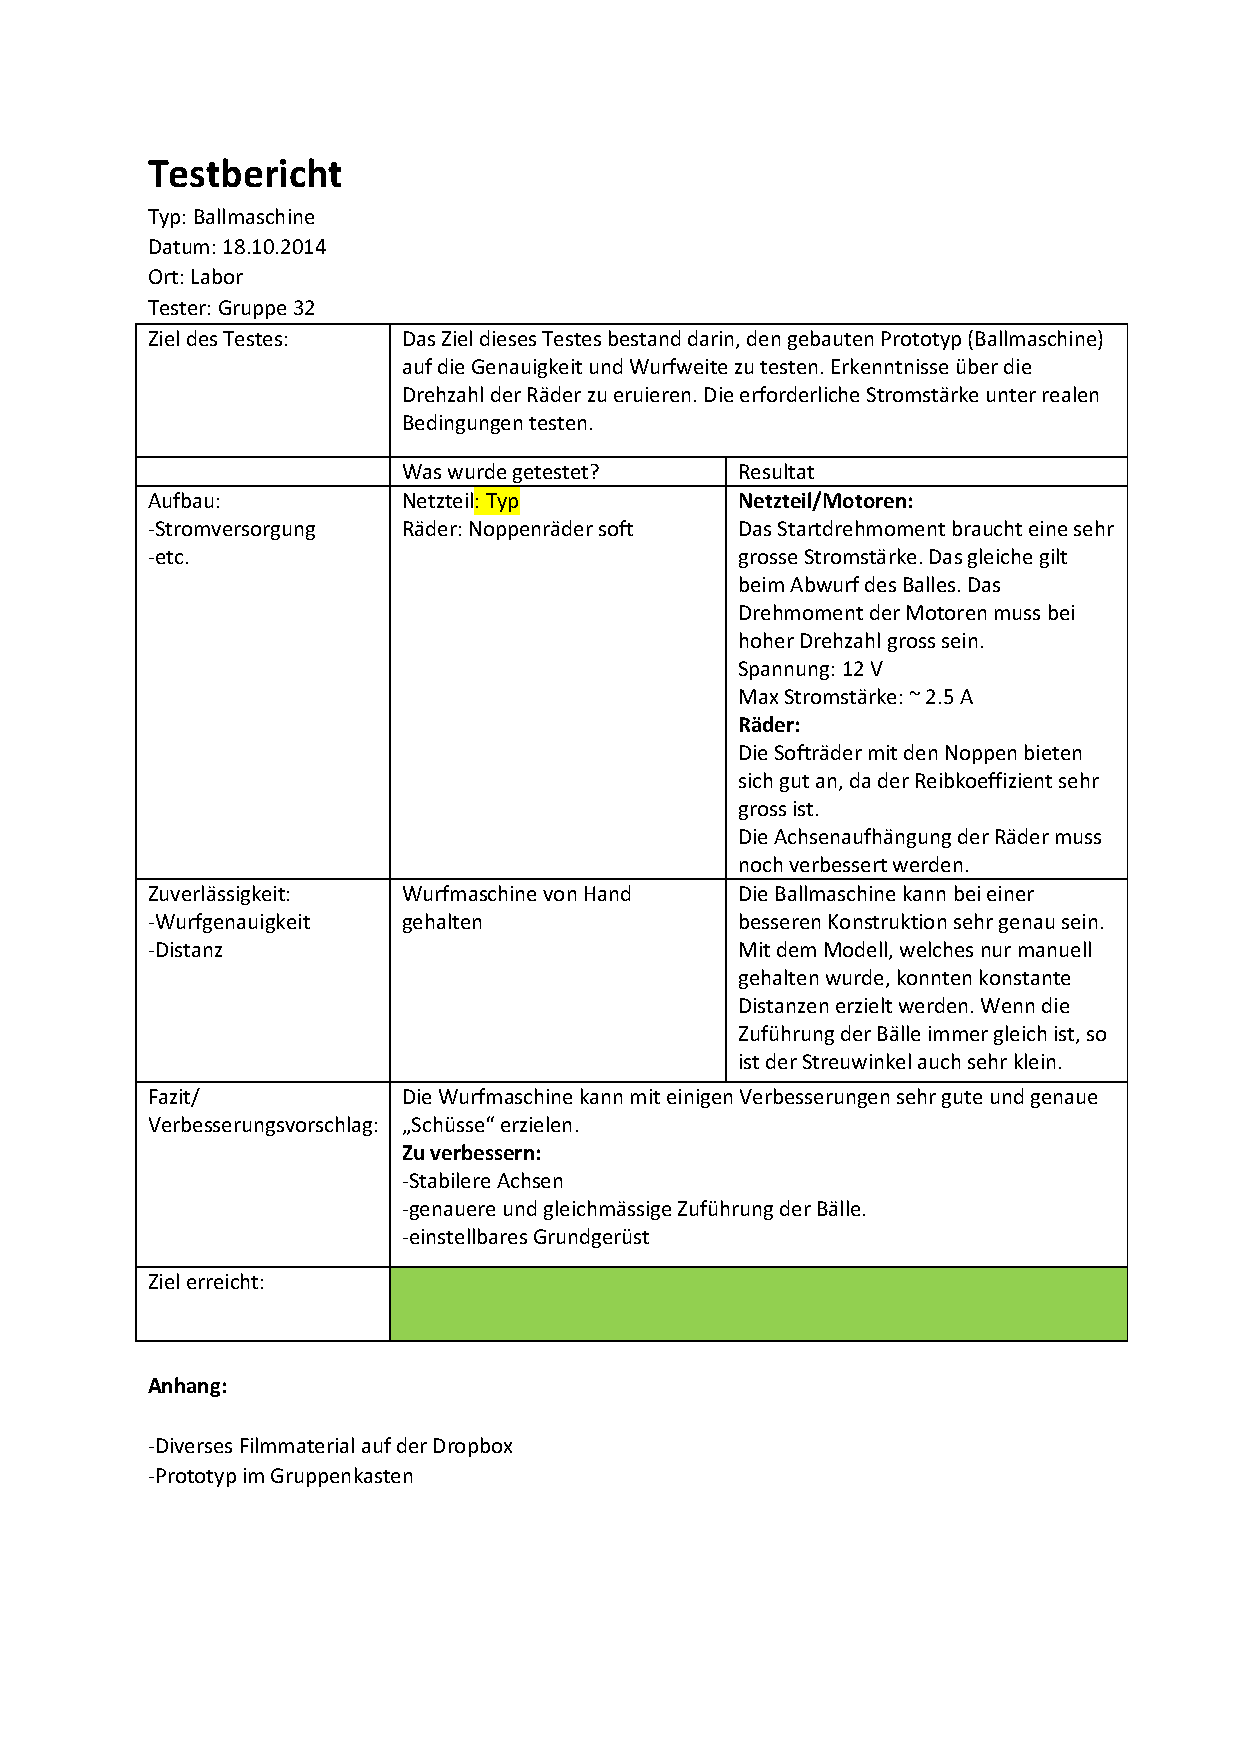
\includegraphics[width=1\textwidth,clip,trim=0mm 0cm 7cm 0cm] 
    {Funktionstests/Bilder/Ballmaschine.jpg}}
%
\caption{Funktionsmuster Ballmaschine}
\label{fig:Ballmaschine}
\end{figure}
%
%\begin{figure}[h!]
%    \begin{minipage}[hbt]{0.7\textwidth}
%    	\includegraphics[width=1\textwidth,clip,trim=0mm 0cm 7cm 0cm]
%    	{Funktionstests/Bilder/Ballmaschine.jpg}
%    	\centering
%    	\caption{Funktionsmuster Ballmaschine} 
%        \label{abb:Ballmaschine_Drehzahl1}
%    \end{minipage}
%\hfill
%    \begin{minipage}[hbt]{0.3\textwidth}
%    	\includegraphics[width=.9\textwidth,clip,trim=27cm 2cm 0mm 2.5cm]
%    	{Funktionstests/Bilder/Ballmaschine.jpg}
%    	\centering
%    	\caption{Funktionsmuster Front Ansicht} 
%        \label{abb:Ballmaschine_Drehzahl1}
%    \end{minipage}
%\end{figure}